%\documentclass[dvipdfmx]{beamer}      % platex の場合
\documentclass{beamer}                 % lualatex の場合
\usepackage{mySld}

\begin{document}
\title{基礎コンピュータ工学\\第1章 はじめに}
\date{}

\begin{frame}
  \titlepage
\end{frame}

%==============================================================================
%\begin{frame}
%  \frametitle
%  \tableofcontents
%\end{frame}

\section{はじめに}
%==============================================================================
\begin{frame}
  \frametitle{この科目で学ぶこと}
  この科目ではコンピュータの動作原理を学ぶ.
  \vfill
  \begin{itemize}
  \item 1946年にフォン・ノイマンが(Von Neumann)が発明
  \item {\bf ノイマン型コンピュータ}と呼ばれる.
  \item スーパーコンピュータから{\bf マイコン}まで全てノイマン型.\\
    (マイコン=マイクロコンピュータ:超小型コンピュータ)
  \item ノイマン型は発明されて70年以上が経過
  \item ノイマン型の時代は,まだ,しばらく続く
  \end{itemize}
  \vfill
  {\bf ノイマン型コンピュータの動作原理}を学ぶことは,
  寿命の長いエンジニアになるために大切なステップ!
\end{frame}

%==============================================================================
\begin{frame}
  \frametitle{教材用コンピュータ}
  TeC(Tokuyama Educational Computer):徳山高専教育用コンピュータ

  \begin{center}
    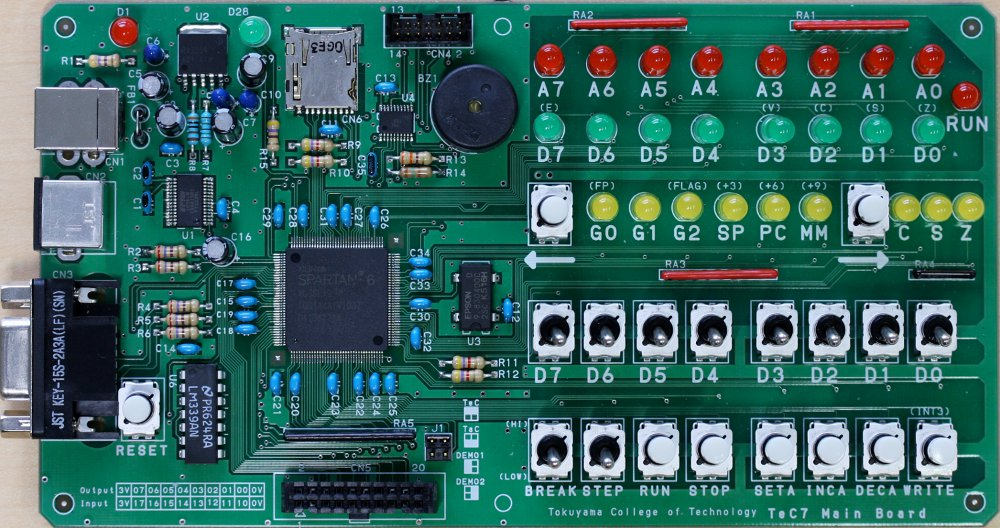
\includegraphics[scale=0.2]{chap1/TeC7.jpg}
  \end{center}

  \begin{itemize}
  \item PCやスマフォは巨大システム
  \item PCやスマフォは動作原理を勉強するには難しすぎる
  \item TeCは動作原理を学ぶために特化し単純・小規模
  \item 学生が所有し,家でも演習ができる.
  \end{itemize}
\end{frame}

\end{document}
